\documentclass[12pt, twoside]{article}
%\documentclass[12pt, twoside]{article}
\usepackage[letterpaper, margin=1in, headsep=0.2in]{geometry}
\setlength{\headheight}{0.6in}
%\usepackage[english]{babel}
\usepackage[utf8]{inputenc}
\usepackage{microtype}
\usepackage{amsmath}
\usepackage{amssymb}
%\usepackage{amsfonts}
\usepackage[nomessages]{fp} %\FPeval{\var-name}{2*sin(pi/6)}
\usepackage{siunitx} %units in math. eg 20\milli\meter
\usepackage{yhmath} % for arcs, overparenth command
\usepackage{tikz} %graphics
\usetikzlibrary{quotes, angles, arrows, arrows.meta}
\usepackage{pgfplots}
\usepgfplotslibrary{fillbetween}
\pgfplotsset{compat=1.16}
\usepackage{graphicx} %consider setting \graphicspath{{images/}}
\usepackage{parskip} %no paragraph indent
\usepackage{enumitem}
\usepackage{multicol}
\usepackage{venndiagram}

\usepackage{fancyhdr}
\pagestyle{fancy}
\fancyhf{}
\renewcommand{\headrulewidth}{0pt} % disable the underline of the header
\raggedbottom
\hfuzz=2mm %suppresses overfull box warnings

\usepackage{hyperref}

\fancyhead[LE]{\thepage}
\fancyhead[RO]{Markscheme}
\fancyhead[LO]{La Scuola d'Italia / Dr.\ Huson / IB Math 11 \\* 19 October 2026}

\begin{document}
\subsubsection*{2 Homework: Slope, Lines and Systems of Equations --- Markscheme}

\begin{enumerate}[itemsep=0.3cm]

%--- Problem 1: Gradient from two points; equation y = mx + c; axis intercepts; point on the line [9 marks] ---
\item[1.] [Maximum mark: 9]

\textbf{(a)} $m = \frac{4 - 1}{4 - (-2)}$ \hfill \textbf{M1}

$m = \frac{3}{6} = \frac{1}{2}$ \hfill \textbf{A1}

\textbf{(b)} $y - 1 = \frac{1}{2}(x + 2)$ \hfill \textbf{M1}

$y = \frac{1}{2}x + 2$ \hfill \textbf{A1}

\emph{Accept $y - 4 = \frac{1}{2}(x - 4)$ for the M1. FT from (a).}

\textbf{(c)} $y$-intercept: $2$ \hfill \textbf{A1}

$0 = \frac{1}{2}x + 2$ \hfill \textbf{M1}

$x = -4$ \hfill \textbf{A1}

\emph{Accept $(0, 2)$ and $(-4, 0)$. FT from (b).}

\textbf{(d)} $k = \frac{1}{2}(10) + 2$ \hfill \textbf{M1}

$k = 7$ \hfill \textbf{A1}

\emph{Accept the gradient method $\frac{k - 4}{10 - 4} = \frac{1}{2}$ for the
M1. FT from (b).}

\medskip

%--- Problem 2: General form 2x + 3y = 12; intercepts, gradient, perpendicular line, parallel line [9 marks] ---
\item[2.] [Maximum mark: 9]

\textbf{(a)} $y = 0$: $2x = 12$, so $x = 6$ \hfill \textbf{A1}

$x = 0$: $3y = 12$, so $y = 4$ \hfill \textbf{A1}

\emph{Accept $(6, 0)$ and $(0, 4)$.}

\textbf{(b)} $3y = -2x + 12$

$y = -\frac{2}{3}x + 4$ \hfill \textbf{M1}

$m = -\frac{2}{3}$ \hfill \textbf{A1}

\emph{Accept the gradient from the intercepts, $\frac{4 - 0}{0 - 6}$, for the
M1.}

\textbf{(c)} $m_{2} = \frac{3}{2}$ \hfill \textbf{A1}

$y - 1 = \frac{3}{2}(x - 4)$ \hfill \textbf{M1A1}

\emph{Accept $y = \frac{3}{2}x - 5$ or $3x - 2y = 10$. FT from (b): the
gradient of $L_{2}$ is the negative reciprocal of the candidate's gradient.}

\textbf{(d)} $y = -\frac{2}{3}x - 2$ \hfill \textbf{A1A1}

\emph{A1 for the gradient $-\frac{2}{3}$, A1 for the intercept $-2$. Accept
$2x + 3y = -6$. FT from (b).}

\newpage

%--- Problem 3: Solve two 2x2 systems by hand (substitution, elimination) [6 marks] ---
\item[3.] [Maximum mark: 6]

\textbf{(a)} $3x + 2y = 16$, \; $x - y = 2$.

$x = y + 2$

$3(y + 2) + 2y = 16$ \hfill \textbf{M1}

$5y + 6 = 16$

$y = 2$ \hfill \textbf{A1}

$x = 2 + 2 = 4$ \hfill \textbf{A1}

\emph{Accept elimination: $2x - 2y = 4$ added to $3x + 2y = 16$ gives
$5x = 20$. Correct values with no working earn 1 mark: the question asks
for working.}

\textbf{(b)} $2x + 3y = 7$, \; $5x - 2y = -11$.

$4x + 6y = 14$

$15x - 6y = -33$ \hfill \textbf{M1}

$19x = -19$

$x = -1$ \hfill \textbf{A1}

$2(-1) + 3y = 7$

$3y = 9$

$y = 3$ \hfill \textbf{A1}

\emph{M1 for multiplying to match the coefficients of one variable, or for
a correct substitution. Correct values with no working earn 1 mark.}

\newpage

%--- Problem 4: Read equation of a graphed line; graph x + y = 7; mark and state intersection; solve algebraically [9 marks] ---
\item[4.] [Maximum mark: 9]

\begin{minipage}[t]{0.53\linewidth}
\vspace{0pt}
\begin{tikzpicture}[scale=0.6]
  \draw [thin, color=gray, xstep=1.0cm, ystep=1.0cm] (-2.5,-4.5) grid (8.5,8.5);
  \foreach \x in {-2,-1,0,1,2,3,4,5,6,7,8}
    \node[below] at (\x,-4.5) {$\x$};
  \foreach \y in {-4,-3,-2,-1,0,1,2,3,4,5,6,7,8}
    \node[left] at (-2.5,\y) {$\y$};
  \draw [thick, ->] (-2.5,0) -- (8.9,0) node [right] {$x$};
  \draw [thick, ->] (0,-4.5) -- (0,8.9) node [right] {$y$};
  % Line L: y = (3/2)x - 3 (given)
  \draw [very thick] (-1,-4.5) -- (7.667,8.5) node [right] {$L$};
  % Line M: x + y = 7 (student draws)
  \draw [very thick, dashed] (-1.5,8.5) -- (8.5,-1.5) node [right] {$M$};
  % Intersection (4, 3); label in the gap left of the point, between M and L
  \node[circle, fill, inner sep=1.5pt] at (4,3) {};
  \node[left] at (3.2,3) {$(4, 3)$};
\end{tikzpicture}
\end{minipage}
\hfill
\begin{minipage}[t]{0.45\linewidth}
\vspace{0pt}
\textbf{(a)} $y = \frac{3}{2}x - 3$ \hfill \textbf{A1A1}

\emph{A1 for the gradient $\frac{3}{2}$, A1 for the intercept $-3$. The
line passes through $(0, -3)$, $(2, 0)$ and $(4, 3)$.}

\textbf{(b)} $M$ through $(0, 7)$, $(7, 0)$ \hfill \textbf{A1A1}

\emph{A1 for each correct intercept, joined by a straight ruled line.}

\textbf{(c)} $(4, 3)$, marked \hfill \textbf{A1A1}

\emph{A1 for the point marked, A1 for the ordered pair. FT from the
candidate's line $M$.}
\end{minipage}

\medskip

\textbf{(d)} $x + \left(\frac{3}{2}x - 3\right) = 7$ \hfill \textbf{M1}

$\frac{5}{2}x - 3 = 7$

$\frac{5}{2}x = 10$

$x = 4$ \hfill \textbf{A1}

$y = 7 - 4 = 3$ \hfill \textbf{A1}

\emph{FT from the candidate's equation in (a). Accept $\frac{3}{2}x - 3 = 7 - x$
for the M1.}

\end{enumerate}
\end{document}
